\section{Performance Measurement}


\subsection{flips and flops}

\paragraph{flips}  This is intended to measure \emph{instruction} rate through 
the floating point pipe with no massaging.



\paragraph{flops}  Perhaps the more well-known measurement is the rate of  
floating point \emph{operations}.  



\paragraph{Theoretical flops}
\begin{align*}
\text{flops} = \text{(\# cores)} * \text{(\# of SSE units per core)} *  
\text{(cycles / second)} * \text{(\# SSE operations per cycle)}
\end{align*}

single precision (divide by 2 for double precision).

So for this Intel Sandy Bridge Core i5 as a reference, the 

\begin{align*}
\text{Mflops} &= (4) * (2) * (3200 Mhz) * 2 \\ 
&= 25600 
\end{align*}

or about 25 Gflops (25,000,000,000 flops), aka, a hell of a lot of arithmetic.




\subsection{Cache Misses and Cache Hits}

\paragraph{Memory and Cache}

Computers operate at \emph{billions} of cycles per second.  Of course, those  
operations occur on data.  A useful abstraction we use in thinking about 
processing data is you load the stuff up into ram and then the processor does 
things to it.  This is usually fine, or at least convenient, but it's not 
accurate, as you are probably aware.  

\begin{figure}[ht]
  \centering
  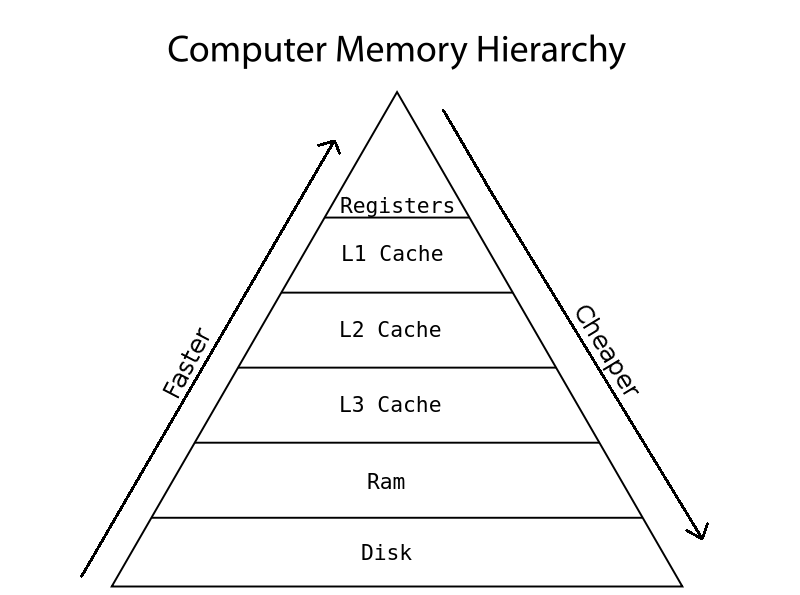
\includegraphics[scale=.54]{./include/pics/memory}
  \caption{Memory Hierarchy}
  \label{fig:mem}
\end{figure}
Another more accurate abstraction is that shown in Figure~\ref{fig:mem}.  In a 
sense, the magic really happens when things get into the CPU registers.  But 
something that's in ram that you want to operate on, as it's headed to the CPU, 
it gets cached into various levels of (comparatively) fast access storage along 
the way. Not understanding this (simplified from reality) architecture can have 
can cause some pretty nasty performance side-effects. on your code.
% \begin{figure}[ht]
%   \centering
%   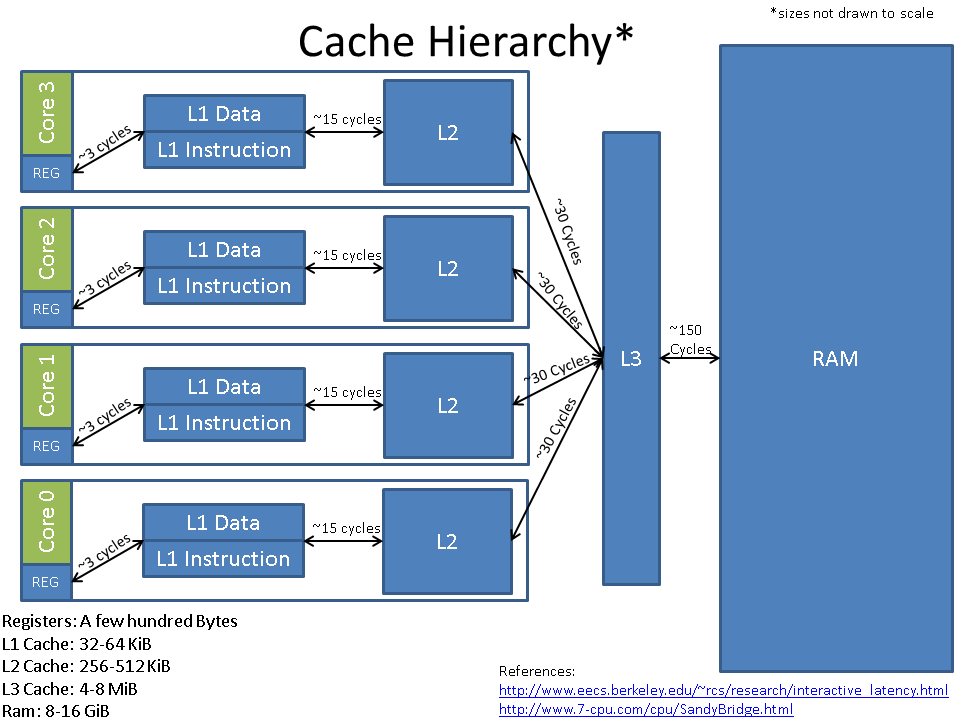
\includegraphics[width=.9\textwidth]{./include/pics/cache}
%   \caption{Still from Interactive Visualization Showing Relative Memory Access Speeds}
%   \label{fig:cache}
% \end{figure}
If you're unfamiliar with this, I would strongly encourage you to check out 
this really cool interactive
\href{http://www.overbyte.com.au/misc/Lesson3/CacheFun.html}{visualization} 
showing (relative) speeds of cache misses, also shown in Figure~\ref{fig:cache}. 
It too involves some hefty simplifications of how modern hardware actually 
works, so if this is at all confusing, let us all take a moment to pity the 
tragic life of the computer engineer.


\href%
  {http://www.eecs.berkeley.edu/~rcs/research/interactive_latency.html}%
  {Latency Numbers}





\paragraph{Cache Misses} Fundamentally, a cache miss occurs when the cache 
needs some piece of data to pass along to registers, but it isn't immediately 
available and has to go digging through ram (or god help you, disk) to get it.  
Cache misses are bad and reduce performance.  You can't get rid of them, unless 
your entire problem fits into cache (which is glorious when it happens), but you 
can eliminate \emph{unnecessary} cache misses being aware of how your data and 
algorithms interact with cache.  When people tell you things like ``R's matrices 
are column-major'' or that you should loop over columns then rows, this is 
exactly what they are talking about.
